根据题意，玩家停留和移动都需要消耗物资，可在起点和村庄购买物资，在矿山处可以挖矿赚取资金，但沙尘暴天气无法前进，最后可以在终点处退还剩余的物资换取资金。
%
玩家需要在30天内从起点出发，最终到达终点，要求最大化最终的金额。梳理题目中的所有要求，画出题目示意图。

\begin{figure}[H] % 参数 h(here), t(top), b(bottom), p(page) 控制浮动位置
    \centering % 使图片居中
    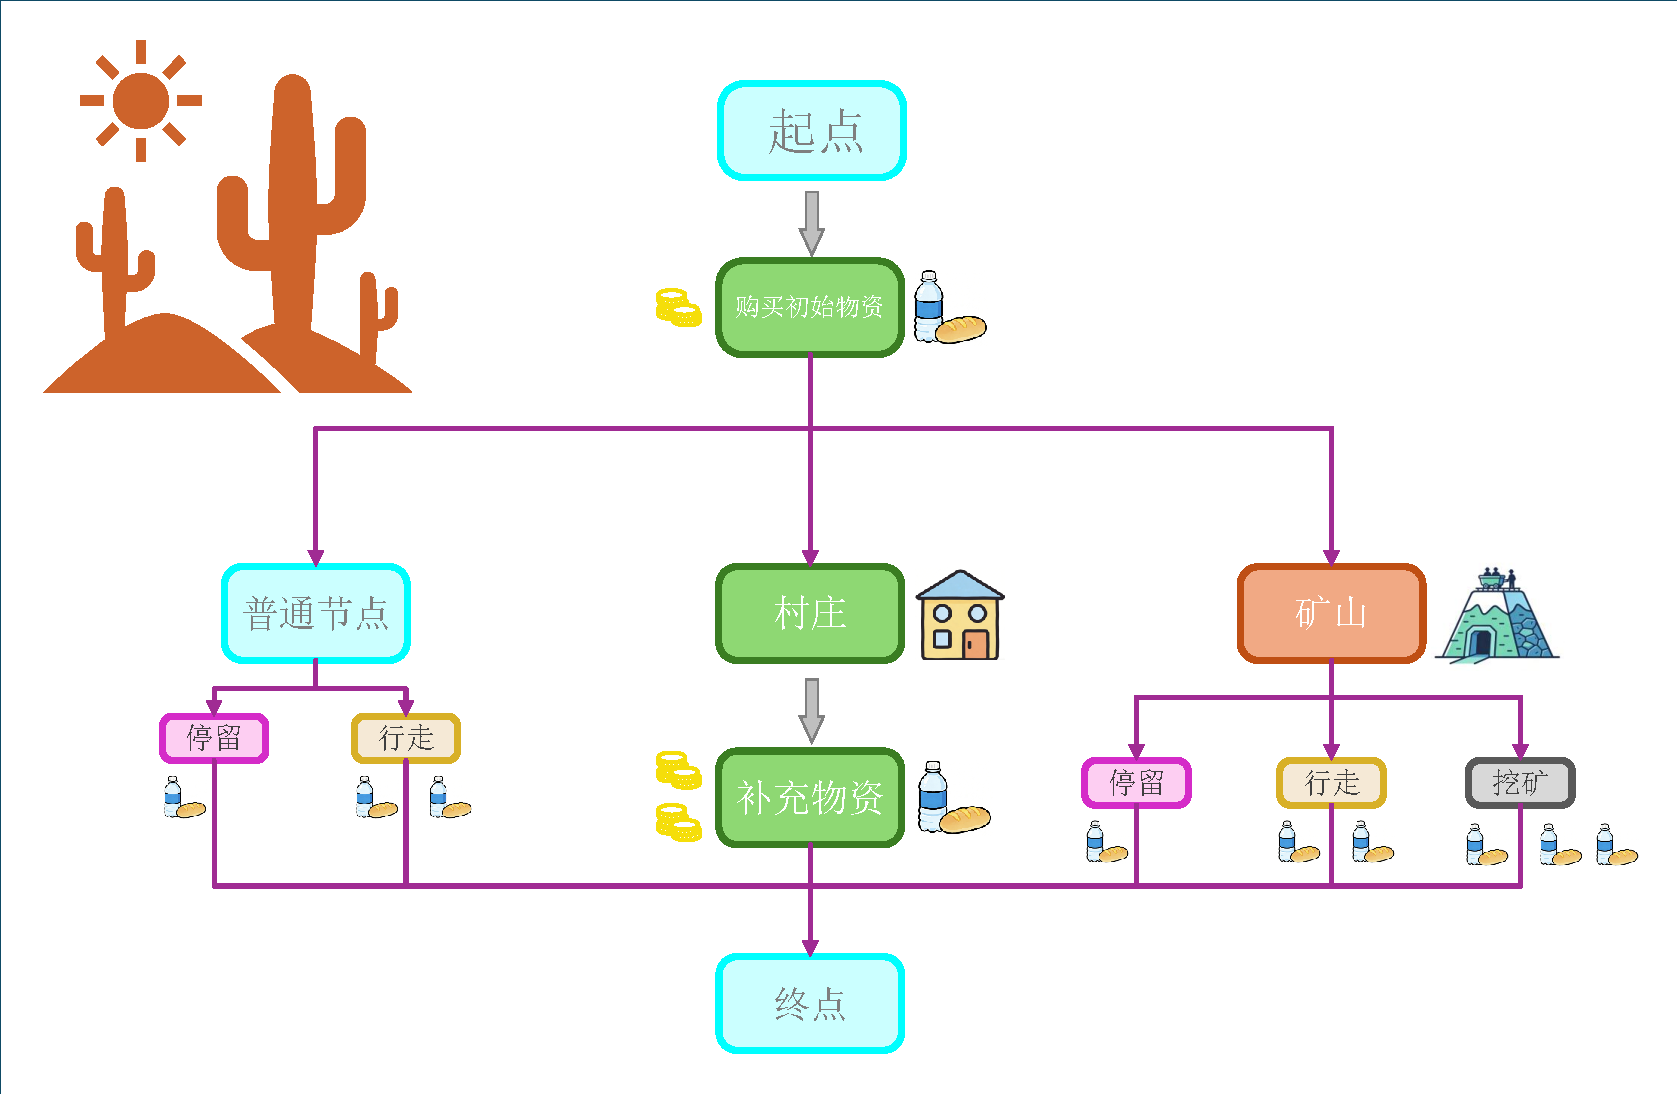
\includegraphics[width=0.8\textwidth]{C2020b/figure/题目示意图.pdf}
    \caption{题目示意图} % 图片标题
\end{figure}

\subsubsection{在已知天气情况时一名玩家的最佳策略模型的建立：}
\noindent\ding{70} \textbf{最简地图模型的建立}：

为了简化后续动态规划的复杂度，我们先对题目所给出的图进行简化，把每个区域看成一个点，把区域相邻的条件看成两个区域之间有一条无向边，由此对地图进行重构。

观察题目可以发现，去往矿山和村庄等重要节点时，在走的天数相同的情况下，消耗金额只和天气相关，所以我们可以直
%
接计算出起点、村庄、矿山和终点两两之间的最短距离。求最短路径的算法我们采用Dijkstra算法进行求解。\\

\noindent\ding{70} \textbf{停留地点的选择：}

    由题意可知，玩家可以在任意地点停留，但是经过分析，我们认为除了沙暴天必须停留外，只有在矿
    %
    山处停留才会获得收益，在其它节点处停留只会带来较大的亏损：带来较大亏损；设 $P_B$ 为参与者挖矿获得的基础
    %
    收益，$P_W$、$P_F$ 分别为水和食物的基础价格，下面我们对这两种情况进行具体的分析和说明。

    \ding{111} \textbf{矿山挖矿必定获得收益}

    若参与者在矿山挖矿一天，则这一天他将多消耗一部分水和食物，同时也会晚一天到达终点；我们按照最坏情况进行计算
    %
    ，即他挖矿的那一天遭遇了沙暴天气，同时在第17天到达终点前一个结点，根据第一关、第二关的参数设定，此时每天食物
    %
    和水的基础消耗量均为10箱，同时最后一天其消耗量为基础消耗量的两倍，因此他的收益为
    \[
    P_1 = P_B - \left(10P_W + 10P_F\right) - 2\left(10P_W + 10P_F\right) - 2\left(8P_W + 6P_F\right),
    \]
    该式的第二项为相比于正常行进，参与者在沙暴天气挖矿所需多消耗的生活必需品对应的资金；由于参与者在第17天到达终
    %
    点前一个结点，因此他需要在该结点等待两天，在第三天再前往终点，第三项、第四项即为这三天他所需多消耗的生活必需品
    %
    对应的资金。经过整理化简，并代入题中所给数据，可得 $P_1 = 350 > 0$，由于该情况为最坏情况，所以我们可以得出
    %
    结论：参与者挖矿必定获得收益。

    \ding{111} \textbf{其他节点停留必定带来亏损}

    若参与者在其他地点停留，且停留的那天未遭遇沙暴，我们按照最好情况进行计算，即停留的那天以及到
    %
    达终点的那一天的天气均是晴朗，则其因为停留导致的亏损为
    \[
    P_2 = \left(5P_W + 7P_F\right) + 2\left(5P_W + 7P_F\right),
    \]
    该式的第一项为参与者因为在该结点停留所需消耗的生活必需品对应的资金，第二项为参与者晚到终点一天所需
    %
    多消耗的生活必需品对应的资金；经过整理化简，并代入题中所给数据，可得 $P_2 = 285 > 0$，由于该情况为
    %
    最好情况，所以我们可以得出结论：参与者在其余地点停留必定导致亏损。

\noindent\ding{70} \textbf{物资剩余量以及剩余资金的递推关系式}

当我们在起始点准备出发的时候，我们要先购买物资，所以在起点处购买物资后的剩余资金：
\[
G_1 = G_0 - [P_w * B_w + P_f * B_f] 
\]

根据我们上面的分析，我们可以知道参与者只会在矿山处停留，所以我们仅给出向前行走，
%
沙暴天停留，矿山处挖矿和村庄补给下的物资以及剩余资金的递推关系式

\ding{80} \textbf{向前行走时物资剩余量的递推关系式：}

设第t天水的消耗量为$\hat c_w(D_t)$，食物的消耗量为$\hat c_f(D_t)$,由于行走的消耗量是基础消耗量的两倍，所以第$t$天的物资数量为：
\[
\left\{
\begin{aligned}
&W_t=W_{t-1}-2c_w(D_t), \qquad t=1,2,\dots,\tau, \\[1mm]
&F_t=F_{t-1}-2c_f(D_t), \qquad t=1,2,\dots,\tau. \\[1mm]
\end{aligned}
\right.
\]
此时剩余资金不发生变化，即：
\[G_t = G_{t - 1}\]

\ding{80} \textbf{沙暴天停留时物资剩余量的递推关系式：}

根据游戏规则，在遭遇沙暴天时必须做出停留的决策，此时停留的消耗量即为基础消耗量，所以第$t$天的物资数量为：
\[
\left\{
\begin{aligned}
&W_t=W_{t-1}-c_w(D_t), \qquad t=1,2,\dots,\tau, \\[1mm]
&F_t=F_{t-1}-c_f(D_t), \qquad t=1,2,\dots,\tau. \\[1mm]
\end{aligned}
\right.
\]
剩余资金同上。

\ding{80} \textbf{矿山挖矿时物资剩余量的递推关系式：}

如果玩家在矿山进行挖矿决策，那么他挖矿的消耗量是基础物资的三倍，所以第$t$天的物资数量为：
\[
\left\{
\begin{aligned}
&W_t=W_{t-1}-3c_w(D_t), \qquad t=1,2,\dots,\tau, \\[1mm]
&F_t=F_{t-1}-3c_f(D_t), \qquad t=1,2,\dots,\tau. \\[1mm]
\end{aligned}
\right.
\]
其中，
\[
r(a_t)=
\begin{cases}
R_0, & a_t=\text{mine},\\
0, & \text{otherwise},
\end{cases}
\]
在挖矿时玩家会获得一定的收益，所以有：
\[G_t = G_{t - 1} + r(a_t)\]

根据以上三种情况我们把公式进行整合：
\[
\left\{
\begin{aligned}
&W_t=W_{t-1}-c_w(D_t,a_t), \qquad t=1,2,\dots,\tau, \\[1mm]
&F_t=F_{t-1}-c_f(D_t,a_t), \qquad t=1,2,\dots,\tau. \\[1mm]
\end{aligned}
\right.
\]
其中
\[
c_w(D_t,a_t)=
\begin{cases}
2\,\hat c_w(D_t), & a_t=\text{move},\\
\hat c_w(D_t), & a_t=\text{stay},\\
3\,\hat c_w(D_t), & a_t=\text{mine},
\end{cases}
\qquad
c_f(D_t,a_t)=
\begin{cases}
2\,\hat c_f(D_t), & a_t=\text{move},\\
\hat c_f(D_t), & a_t=\text{stay},\\
3\,\hat c_f(D_t), & a_t=\text{mine}.
\end{cases}
\]

\ding{80} \textbf{村庄补给时物资剩余量的递推关系式：}

设玩家在村庄购买水的数量为$B_t^w$箱，购买的食物数量为$B_t^f$箱，又因为玩家在村庄无需停留，所以其物资消耗量是基础消耗量的两倍。所以第$t$天的物资数量为：
\[
\left\{
\begin{aligned}
&W_t=W_{t-1}-2*c_w(D_t,a_t)+B_t^w, \qquad t=1,2,\dots,\tau, \\[1mm]
&F_t=F_{t-1}-2*c_f(D_t,a_t)+B_t^f, \qquad t=1,2,\dots,\tau. \\[1mm]
\end{aligned}
\right.
\]
在补给物资时需要消耗资金，且村庄售价为基础物资的两倍，所以剩余资金为：
\[G_t = G_{t - 1} - 2*[P_wB_t^w+P_fB_t^f] \]

我们把在村庄购买和在起始点购买的情况进行整合：
\[
G_t=G_{t-1}-p_t^wB_t^w-p_t^fB_t^f
\]
其中，
\[
p_t^w=
\begin{cases}
P_w, & t=0,\ N_0=N_s,\\
2P_w, & N_{t-1}\in\Omega_v,\\
0, & \text{otherwise},
\end{cases}
\qquad
p_t^f=
\begin{cases}
P_f, & t=0,\ N_0=N_s,\\
2P_f, & N_{t-1}\in\Omega_v,\\
0, & \text{otherwise}.
\end{cases}
\]

综上所述,考虑到物资的购买和消耗，剩余资金的增加和减少可得出：
\[
\left\{
\begin{aligned}
&W_t=W_{t-1}+B_t^w-c_w(D_t,a_t), \qquad t=1,2,\dots,\tau,\\[1mm]
&F_t=F_{t-1}+B_t^f-c_f(D_t,a_t), \qquad t=1,2,\dots,\tau,\\[1mm]
&G_t=G_{t-1}-p_t^wB_t^w-p_t^fB_t^f+r(a_t), \qquad t=1,2,\dots,\tau.\\[1mm]
\end{aligned}
\right.
\]

\noindent\ding{70} \textbf{最佳策略的单目标优化模型}

根据游戏规则，我们建立了单目标的最优化模型：

\ding{78}\textbf{目标函数：剩余资金最多：}

题目要求我们保留最多的资金，所以目标函数为：

\[
\max \ S_1
=G_{\tau}+\frac{1}{2}P_wT_{\tau}+\frac{1}{2}P_fF_{\tau}
\]

其中$G_{\tau}$表示到达终点那一天的剩余资金，$\frac{1}{2}P_wT_{\tau}+\frac{1}{2}P_fF_{\tau}$表示多余物资在终点退回的金额。

\ding{78}\textbf{约束条件1：在截止日期前到达终点}

根据游戏规则，玩家需在规定时间内到达终点，所以有一个约束条件为：

\[
\qquad 0\le \tau \le T_{\max}
\]
其中，$\tau$为到达终点的实际时间，$T_{\max}$为关卡规定的最大时间

\ding{78}\textbf{约束条件2：物资总重量不能超过上限}
设食物的重量为$m_w$,水的重量为$m_f$,参与者的负重上限为$M_{max}$，那么另一个约束条件为：

\[
m_wW_t+m_fF_t\le M_{\max}, \qquad t=0,1,\dots,\tau,\\[1mm]
\]
其中，$W_t$，$F_t$分别是第$t$天水和食物的剩余量。

同时，玩家在去往终点的路程中不能耗尽所有物资，所以：
\[
W_t\ge 0,\quad F_t\ge 0 \qquad t=0,1,\dots,\tau.\\[1mm]
\]

\subsubsection{模型汇总}

则问题一可整理为如下确定性动态优化模型：
\begin{equation}
\max \ S_1
=G_{\tau}+\frac{1}{2}P_wT_{\tau}+\frac{1}{2}P_fF_{\tau}
\label{eq:q1_obj}
\end{equation}
\[
\mathrm{s.t.}\left\{
\begin{aligned}
&N_0=N_s,\qquad N_{\tau}=N_e,\qquad 0\le \tau \le T_{\max},\\[2mm]
&W_t=W_{t-1}+B_t^w-c_w(D_t,a_t), \qquad t=1,2,\dots,\tau,\\[1mm]
&F_t=F_{t-1}+B_t^f-c_f(D_t,a_t), \qquad t=1,2,\dots,\tau,\\[1mm]
&G_t=G_{t-1}-p_t^wB_t^w-p_t^fB_t^f+r(a_t), \qquad t=1,2,\dots,\tau,\\[1mm]
&m_wW_t+m_fF_t\le M_{\max}, \qquad t=0,1,\dots,\tau,\\[1mm]
&W_t\ge 0,\quad F_t\ge 0,\quad G_t\ge 0,\qquad t=0,1,\dots,\tau,\\[1mm]
&a_t=\text{move}\ \Rightarrow\ (N_{t-1},N_t)\in\mathcal{E},\\[1mm]
&a_t=\text{stay}\ \Rightarrow\ N_t=N_{t-1},\\[1mm]
&a_t=\text{mine}\ \Rightarrow\ N_{t-1}\in\Omega_h,\ N_t=N_{t-1},\\[1mm]
&D_t=3\ \Rightarrow\ a_t\neq \text{move},\\[1mm]
&B_t^w,B_t^f\ge 0,\qquad t=0,1,\dots,\tau,\\[1mm]
&B_t^w=B_t^f=0,\qquad N_{t-1}\notin \{N_s\}\cup\Omega_v,\ t\ge 1.
\end{aligned}
\right.
\label{eq:q1_cons}
\]

其中，
\[
c_w(D_t,a_t)=
\begin{cases}
2\,\hat c_w(D_t), & a_t=\text{move},\\
\hat c_w(D_t), & a_t=\text{stay},\\
3\,\hat c_w(D_t), & a_t=\text{mine},
\end{cases}
\qquad
c_f(D_t,a_t)=
\begin{cases}
2\,\hat c_f(D_t), & a_t=\text{move},\\
\hat c_f(D_t), & a_t=\text{stay},\\
3\,\hat c_f(D_t), & a_t=\text{mine},
\end{cases}
\]
\[
r(a_t)=
\begin{cases}
R_0, & a_t=\text{mine},\\
0, & \text{otherwise},
\end{cases}
\qquad
p_t^w=
\begin{cases}
P_w, & t=0,\ N_0=N_s,\\
2P_w, & N_{t-1}\in\Omega_v,\\
0, & \text{otherwise},
\end{cases}
\]
\[
p_t^f=
\begin{cases}
P_f, & t=0,\ N_0=N_s,\\
2P_f, & N_{t-1}\in\Omega_v,\\
0, & \text{otherwise}.
\end{cases}
\]

\subsubsection{在已知天气情况时一名玩家的最佳策略模型的求解：}

\ding{72} \textbf{动态规划模型的求解:}
根据以上的分析，我们采用动态规划算法可以完美适配该模型，所以我们采用动态规划对该方法进行求解。

其中第一、二关中，第t天的食物和水的基础消耗量为：
\[
\hat c_w(D_t)=
\begin{cases}
5, & D_t=1,\\
8, & D_t=2,\\
10, & D_t=3,
\end{cases}
\qquad
\hat c_f(D_t)=
\begin{cases}
7, & D_t=1,\\
6, & D_t=2,\\
10, & D_t=3,
\end{cases}
\]



\textbf{1.数据初始化}

定义一个四维的函数$G(i,j,W,F)$，表示第$i$天，在第$j$个位置下的，水和食物剩余量分别为$W$和$F$时的剩余资金。
%
根据表格数据初始化各天气的食物和水的消耗和路线，设定每个状态的最大收益为无穷小。
%
同时根据第一天的天气给出初始水和食物的购买方案。

\textbf{2.动态规划的求解}

根据上述模型，列出对应的状态转移方程

\textbf{3.结果线路的输出}

利用dfs回溯法来反向寻找经过路线。

\ding{72} \textbf{Dijkstra算法的求解}

为刻画题目中各区域之间的通行关系，本文首先引入 Dijkstra 最短路径算法对地图进行预处理。Dijkstra 算法是一种用于求解非负权图单源最短路径问题的经典算法，适用于边权均为非负的网络结构。将地图抽象为无向赋权图
\[
G=(V,E),
\]
其中，\(V\) 表示地图中所有区域节点的集合，\(E\) 表示节点之间可直接到达的边集合。若节点 \(v_i\) 与节点 \(v_j\) 在地图中相邻，则记 \((v_i,v_j)\in E\)。进一步设边权函数为
\[
w:E\to \mathbb{R}_{\ge 0},
\]
其中，\(w(v_i,v_j)\) 表示从节点 \(v_i\) 移动到节点 \(v_j\) 所需的代价。由于本题中玩家每天最多只能移动到一个相邻区域，且单次移动不存在负代价，故可将相邻区域之间的边权统一记为 1，从而将原问题转化为标准的非负权最短路问题。

Dijkstra 算法的核心思想是“逐步逼近最优解”。设起点为 \(s\)，定义 \(d(v)\) 为起点 \(s\) 到节点 \(v\) 的当前最短距离估计值，初始化为
\[
d(s)=0,\qquad d(v)=+\infty \ \ (v\neq s).
\]
随后，在每一步迭代中，从未确定最短距离的节点中选取具有最小 \(d(v)\) 的节点，将其加入已确定集合，并对其所有邻接节点进行松弛操作：
\[
d(v_j)=\min\{d(v_j),\ d(v_i)+w(v_i,v_j)\}.
\]
重复上述过程，直至所有节点的最短距离均被确定。由于该算法始终在非负权条件下扩展当前最优路径，因此能够保证所得结果即为全局最短路径。该方法不仅可以得到起点到任意节点的最短距离，还可以通过记录前驱节点恢复完整路径序列。

在本题中，Dijkstra 算法主要用于求解起点、村庄、矿山和终点等关键位置之间的最短路径及对应距离，为后续优化模型提供基础数据支持。具体而言，先利用该算法分别计算各关键节点对之间的最短通行路线，得到路径长度与节点经过顺序；再将最短路径结果嵌入后续决策模型中，与天气状态、水和食物消耗、负重约束、补给策略及挖矿收益等因素相结合，进一步建立收益最大化模型。这样处理能够有效减少复杂地图上的无效路径枚举，将“路径搜索”与“资源决策”分层求解，从而提高模型求解效率，并增强整体建模过程的条理性与可解释性。


利用C++编程，我们求解出了第一关和第二关的最优策略和最优收益，结果如下：

\begin{center}
    \begin{tabular}{c|c}
        \hline
        关卡  & 最优收益 \\
        \hline+
        第一关 & 10470 \\
        第二关 & 12730 \\
        \hline
    \end{tabular}
\end{center}

\begin{figure}[H] % 参数 h(here), t(top), b(bottom), p(page) 控制浮动位置
    \centering % 使图片居中
    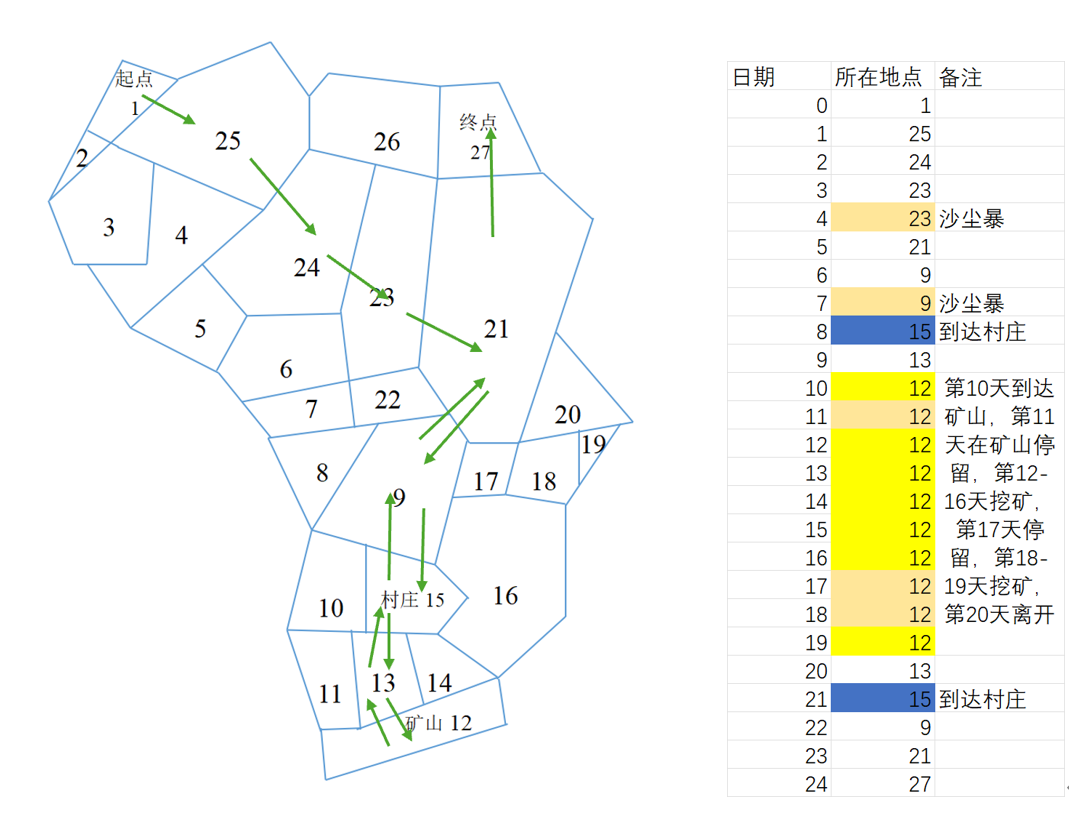
\includegraphics[width=0.8\textwidth]{C2020b/figure/问题一第一关结果图.png}
    \caption{问题一第一关结果图} % 图片标题
\end{figure}

\begin{figure}[H] % 参数 h(here), t(top), b(bottom), p(page) 控制浮动位置
    \centering % 使图片居中
    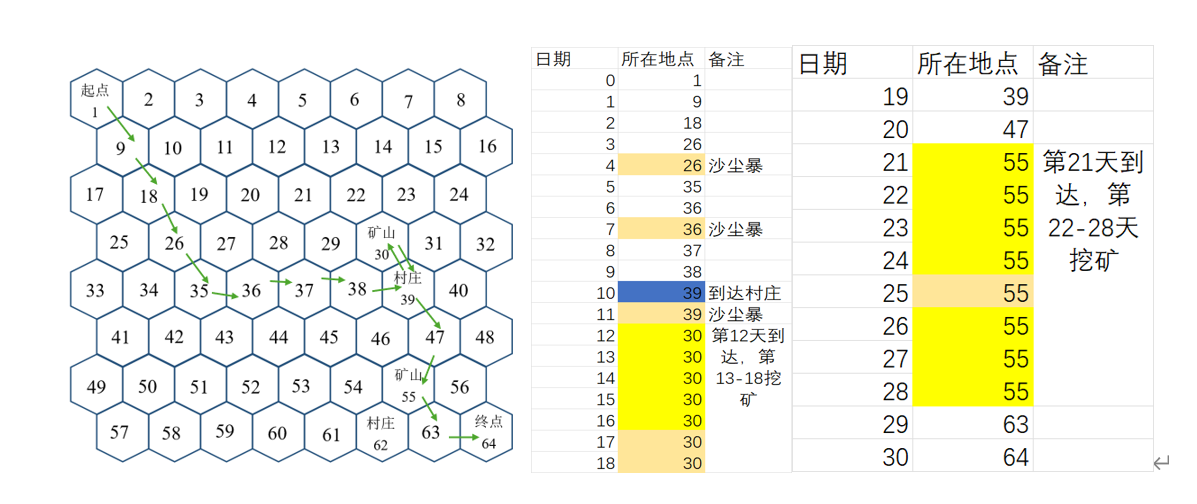
\includegraphics[width=0.8\textwidth]{C2020b/figure/问题一第二关结果图.png}
    \caption{问题一第二关结果图} % 图片标题
\end{figure}